%===============================================================================
\section{Métodos de estimación}
\begin{frame}{Eligiendo un estimador}
	\begin{itemize}
		\item OBJETIVO: Encontrar $\widehat{\beta}$ (estimador de $\beta$) que reduzca el error de estimación. \pause
		\item INCONVENIENTE: Tenemos muchos $u_i$, ¿cómo asumir el valor agregado del error de estimación? \pause
		\item Veamos algunos métodos de estimación
	\end{itemize}
\end{frame}
%===============================================================================

%-------------------------------------------------------------------------------
\subsection{Estimación: Método de momentos}
%-------------------------------------------------------------------------------
\begin{frame}{Estimación: Método de momentos}
	Consiste en igualar momentos poblacionales con muestrales
	\vspace{2mm}
	\begin{block}{$ E(\mu)=0 $}
		Equivalente muestral: $ \sum_{i=1}^{n}(y_{i}-\hat{\beta_{0}}-\hat{\beta_{1}}x_{i})/n=0 $  (I)
	\end{block}
	\begin{exampleblock}{$ E(x \mu)=0 $}
		Equivalente muestral: $ \sum_{i=1}^{n}[x_{i}(y_{i}-\hat{\beta_{0}}-\hat{\beta_{1}}x_{i})]/n=0 $ (II)
	\end{exampleblock}
	De (I) se obtiene:
	$$\overline{y}=\hat{\beta_{0}}-\hat{\beta_{1}}\overline{x} \Leftrightarrow
	\textcolor{red}{\hat{\beta_{0}}=\overline{y}-\hat{\beta_{1}}\overline{x}}$$
	en (II):
	\textcolor{red}{$$\hat{\beta_{1}}=\sum_{i=1}^{n}(x_{i}-\overline{x})(y_{i}-\overline{y})/\sum_{i=1}^{n}(x_{i}-\overline{x})^{2}$$}
	Probar que: \textcolor{red}{$\hat{\beta_{1}}=\rho \sigma_{y}/\sigma_{x}$}
\end{frame}

%-------------------------------------------------------------------------------	
\subsection{Estimación: Mínimos cuadrados ordinarios (MCO)}
%-------------------------------------------------------------------------------
\begin{frame}{Estimación: Mínimos cuadrados ordinarios}
	Dado que se quiere ajustar un grupo de puntos (muestra) a una línea, lo lógico sería entonces minimizar los errores cometidos por tratar de aproximar los puntos por una recta.
		$$\hat Y = \alpha+ \widehat{\beta} X$$
	Error:
		$$\varepsilon_i=Y_i-\hat Y_i=Y_i-(\alpha+\widehat{\beta} X)$$
	Objetivo es minimizar 
		$$\sum_{i=1}^n \varepsilon _i ^2 = \textup{Min} \sum_{i=1}^{n} (Y_{i}-\hat{Y_{i}})^{2}=\textup{Min} \sum_{i=1}^{n} (Y_{i}-\hat{\beta}_{0}-\hat{\beta}_{1}X_{i})^{2}$$
	¿por qué no minimizar los errores sin ninguna potencia? ¿y con otra potencia? ¿y si se minimizan los valores absolutos?
\end{frame}
%---------------------------------------------------
\begin{frame}{MCO simple}
	\begin{itemize}
		\item Modelo Poblacional
		$$y=\beta_{0}+\beta_{1}x+\mu$$
		\item Modelo muestral
		$$\widehat{y}=\widehat{\beta}_{0}+\widehat{\beta}{1}x+\epsilon$$
		\item Ecuaciones normales: $\sum \epsilon_{i}=0$; $\sum \epsilon_{i}x_{i}=0$
		\item Pendiente
		$$\textcolor{red}{\widehat{\beta}_1 = \frac{\sum (x_{i}-\overline{x})(y_{i}-\overline{y})}{\sum (x_{i}-\overline{x})^2}=\frac{\sum (x_{i}-\overline{x})y_{i}}{\sum (x_{i}-\overline{x})^2}}$$
		\item Intercepto
		$$\textcolor{red}{\widehat{\beta}_{0}=\overline{y}-\widehat{\beta}_{1}\overline{x}}$$
	\end{itemize}
\end{frame}
\begin{frame}{Valores predichos y residuales}
	Una vez tengamos las estimaciones (basados en la data, porsupuesto) podemos calcular los valores predichos ($\widehat{y}$) y los residuos ($\widehat{u}$)
	\begin{gather*}
		\widehat{y}_ = \widehat{\beta}_0 + \widehat{\beta}_1x\\
		\widehat{u} = y - \widehat{y}
	\end{gather*}
	El término de error y los residuales no son lo mismo. El primero está asociado al PGD; este último asociado al estimador (hecho por mortales)
\end{frame}
%---------------------------------------------------
\begin{frame}{¿Cómo obtenemos las estimaciones de MCO}
	Consideremos la siguiente data de corte transversal (notas sobre el cuestionario 1). Descargar la data \href{https://econweb.rutgers.edu/frojas/teaching/undergraduate/grades_data.xlsx}{\textcolor{red}{quí}}
	
	\begin{table}
		\centering
		\begin{tabular}{cccccc}
			i & $y_i$ & $x_i$ & $(x_i - \overline{x})$ & $(x_i - \overline{x})^2$ & $(y_i - \overline{y})$ \\
			\hline
			1 & 4.4 & 3 & {} & {} & {}\\
			2 & 4.1 & 3 & {} & {} & {}\\
			3 & 5.2 & 5 & {} & {} & {}\\
			4 & 2.7 & 3 & {} & {} & {}\\
			$\vdots$ & $\vdots$ & $\vdots$ & $\vdots$ & $\vdots$ & $\vdots$ \\
			80 & 3.1 & 4 & {} & {} & {} \\
			\hline
		\end{tabular}
	\end{table}
\end{frame}
%---------------------------------------------------
\begin{frame}{¿Cómo obtenemos las estimaciones de MCO?}
	Una vez que tengamos las estimaciones para $\beta_0$ y $\beta_2$ podemos completar la siguiente tabla.
	\begin{table}
		\centering
		\begin{tabular}{cccccc}
			i & $y_i$ & $x_i$ & $\beta_0$ & $\beta_1x_i$ & $\widehat{y}_i$ \\
			\hline
			1 & 4.4 & 3 & {} & {} & {}\\
			2 & 4.1 & 3 & {} & {} & {}\\
			3 & 5.2 & 5 & {} & {} & {}\\
			4 & 2.7 & 3 & {} & {} & {}\\
			$\vdots$ & $\vdots$ & $\vdots$ & $\vdots$ & $\vdots$ & $\vdots$ \\
			80 & 3.1 & 4 & {} & {} & {} \\
			\hline
		\end{tabular}
	\end{table}
	Pero, ¿serán insesgado y eficientes?
\end{frame}

%-------------------------------------------------------------------------------
\subsection{Caso particular: Modelo ingenuo}
%-------------------------------------------------------------------------------
\begin{frame}{Caso particular: Modelo ingenuo}
	Función a minimizar
		$$g(\alpha)=\sum_{i=1}^n \varepsilon _i ^2= \sum_{i=1}^n (Y_i-\alpha)^2$$
	CPO:
		$$\frac{\partial g(\alpha)}{\partial \alpha}=\sum_{i=1}^n \frac{\partial \varepsilon _i ^2}{\partial \alpha}=\sum_{i=1}^n \frac{\partial \varepsilon _i ^2}{\partial \varepsilon_i} \frac{\partial \varepsilon_i}{\partial \alpha}=0$$
	C2O:
		$$\frac{\partial^2 g(\alpha)}{\partial^2 \alpha}>0$$
\end{frame}
%------------------------------------------------
\begin{frame}{Suma de Residuos en modelo ingenuo}
	PGD: $y=b_1+\mu$; $b_1=0.5$
	\begin{figure}
		\centering
		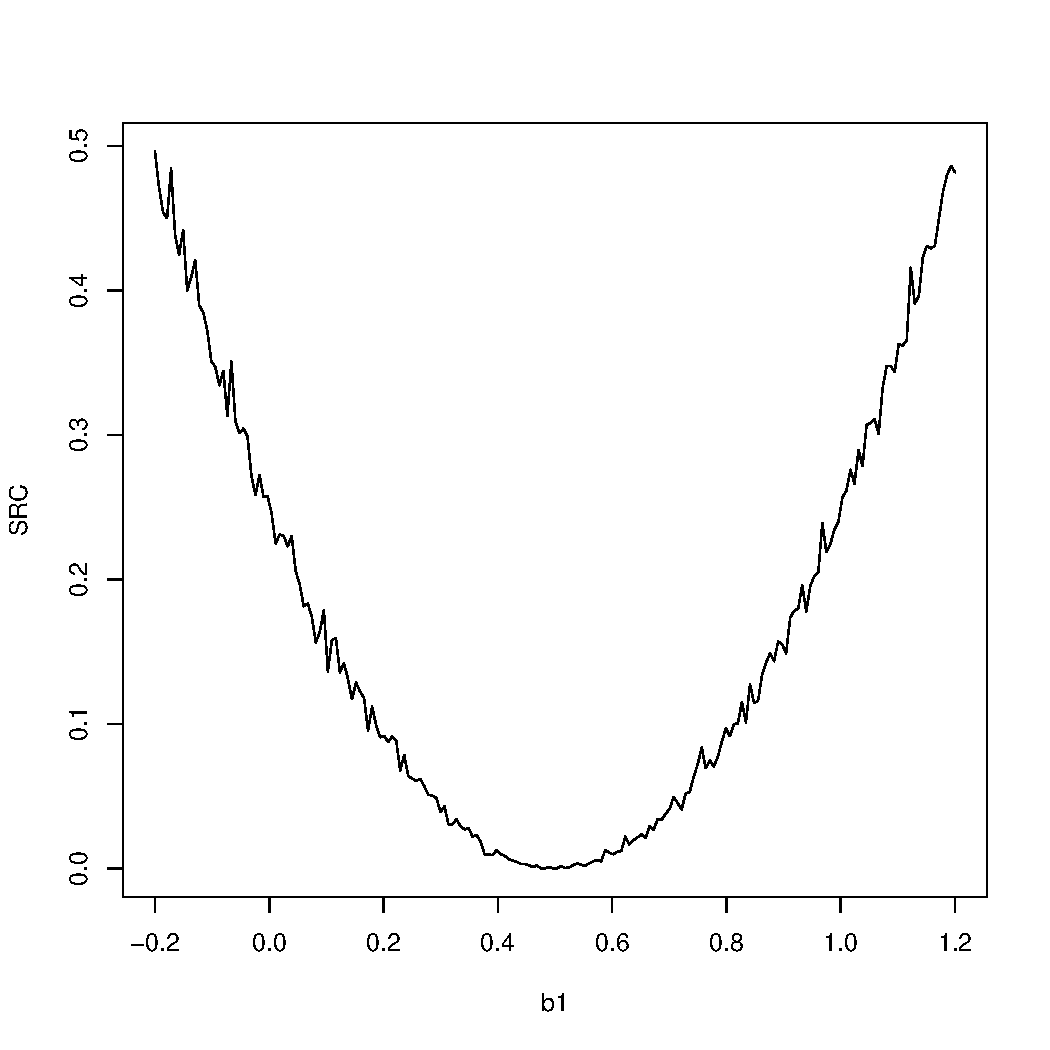
\includegraphics[scale=.38]{fig/SRC0.pdf}
	\end{figure}
\end{frame}

%-------------------------------------------------------------------------------
\subsection{Modelo bivariado}
%-------------------------------------------------------------------------------
\begin{frame}{Modelo bivariado}
	\begin{itemize}
		\item Formalmente ello puede ser obtenido escogiendo $\beta_{0}$ y $\beta_{1}$ tal que minimicen: \\
		$\sum_{i=1}^{n}(\hat{u_{i}})^{2}=\sum_{i=1}^{n}(y_{i}-\hat{\beta_{0}}-\hat{\beta_{1}}x_{i})^{2}$
		\pause
		\item Si uno resuelve el problema de optimización planteando las condiciones de primer orden obtiene: \\
		\textcolor{red}{$ \sum_{i=1}^{n}(y_{i}-\hat{\beta_{0}}-\hat{\beta_{1}}x_{i})=0 $} \\
		\textcolor{red}{$ \sum_{i=1}^{n}[x_{i}(y_{i}-\hat{\beta_{0}}-\hat{\beta_{1}}x_{i})]=0 $}
		\pause
		\item Que es lo mismo que se obtuvo por el método de los momentos
	\end{itemize}
\end{frame}
%------------------------------------------------
\begin{frame}{Suma de Residuos al Cuadrado en modelo bivariado}
	PGD: $y=b_1+b_2x+\mu$;\quad $b_1=0.5$;\quad $b_2=0.2$
	\begin{figure}
		\centering
		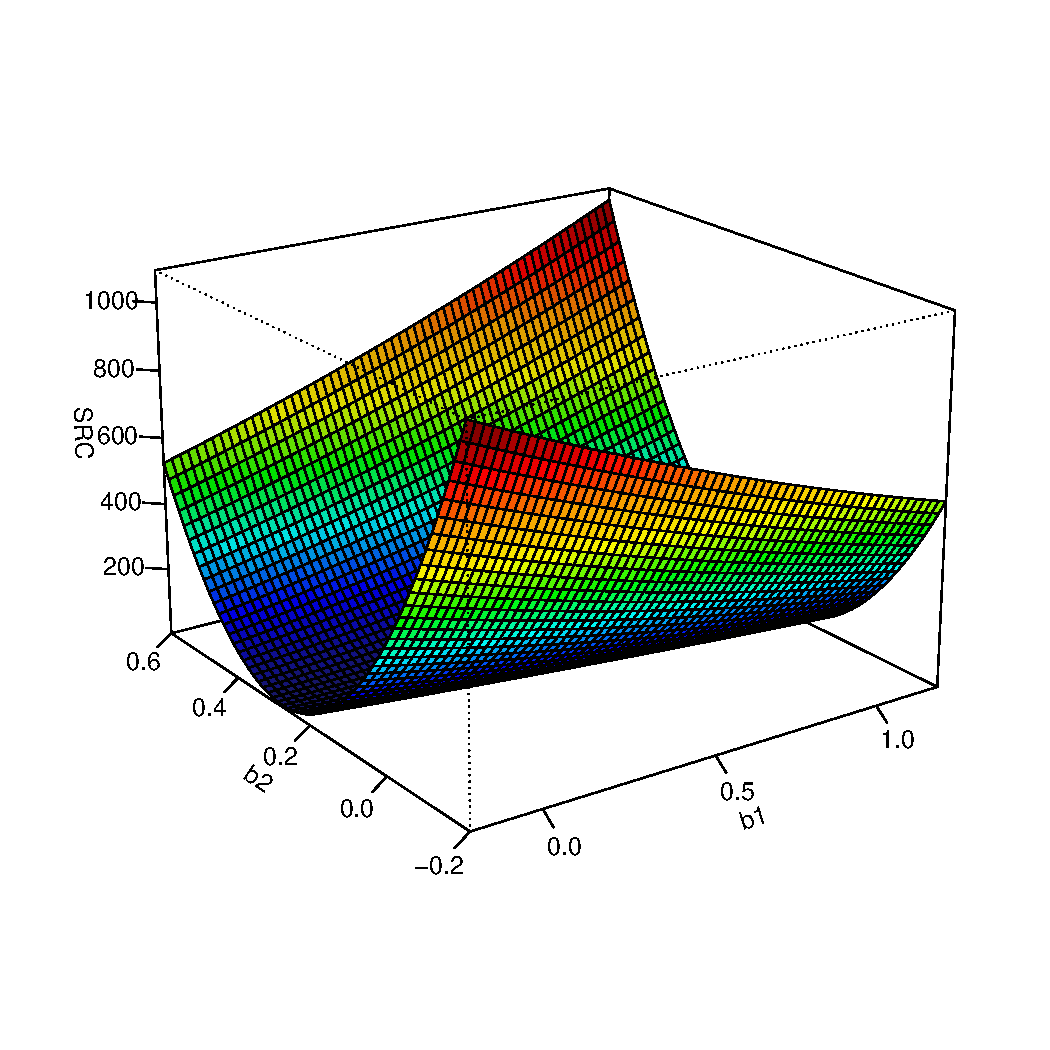
\includegraphics[scale=.38]{fig/SRC.pdf}
	\end{figure}
\end{frame}

